\documentclass{article}
\usepackage{pgf}
\usepackage{tikz}
\usepackage{amsmath, amssymb}
\usetikzlibrary{arrows.meta}
\usetikzlibrary{arrows}
\usetikzlibrary{calc}
\usetikzlibrary{shapes}
\usepackage[utf8]{inputenc}
\begin{document}
    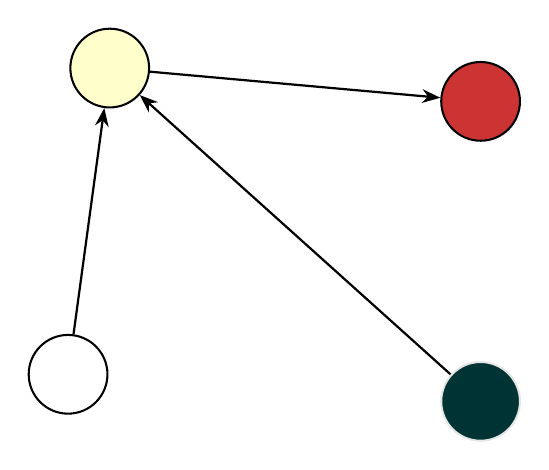
\begin{tikzpicture}[auto]
        \tikzset{>=Stealth}
        \tikzstyle{every path}=[->,thick]
        \tikzstyle{every node}=[ellipse,fill=white,draw=black,text=black,thin,minimum width=1.0cm,minimum height=1.0cm,inner sep=1.5pt]
        \tikzset{quadratic bezier/.style={ to path={(\tikztostart) .. controls($#1!1/3!(\tikztostart)$)
        and ($#1!1/3!(\tikztotarget)$).. (\tikztotarget)}}}

        \definecolor{gfillcolor}{HTML}{FFFFCC}
        \node [fill=gfillcolor, line width=0.026cm] (n0) at (5.006cm,-2.493cm) {};
        \definecolor{gfillcolor}{HTML}{CC3333}
        \node [fill=gfillcolor, line width=0.026cm] (n1) at (9.716cm,-2.916cm) {};
        \definecolor{gfillcolor}{HTML}{003333}
        \definecolor{gstrokecolor}{HTML}{E6E6E6}
        \node [fill=gfillcolor, draw=gstrokecolor, line width=0.026cm] (n2) at (9.716cm,-6.726cm) {};
        \node [line width=0.026cm] (n3) at (4.477cm,-6.382cm) {};

        \draw (n2) to (n0);
        \draw (n0) to (n1);
        \draw (n3) to (n0);
    \end{tikzpicture}
\end{document}
